\chapter{\xlabel{Examples}Examples of Different Reductions}
\label{sec:eg}

\section{\xlabel{Cosmology}Deep point-source maps}
\label{sec:cosmology}

The science goal of many extra-galactic SCUBA-2 observations is to
detect unresolved point sources. In the examples below we work through the
reduction of just such an extra-galactic field, A1835.

Most extra-galactic objects are on average only slightly brighter than
the confusion limit---the fluctuations of the background sky
brightness due to multiple super-imposed, unresolved sources within
the telescope beam, below which individual sources cannot be detected.
It is likely that any sources in the map will be at best, only a few
standard deviations brighter than the noise in the map (caused by a
combination of instrumental noise and source confusion).

\subsection{Example 1 -- The simple reduction}
The basic reduction method for maps like these follow two main
steps---running the data through the map-maker using the
\file{dimmconfig\_blank\_field.lis} configuration file (see
\cref{Section}{sec:config}{Specialised configuration files}). Then
applying the \picard\ \drrecipe{SCUBA2\_MATCHED\_FILTER} recipe (see
\cref{Section}{sec:mf}{Point-source extraction}).
\\ \\
\textbf{Step 1: Run the map-maker}\\
In this example the raw data are stored locally in a directory called
\file{data}. We have three observations (\#13, \#18, \#21) of the field
which we will reduced independently.

\begin{terminalv}
% makemap data/s8*00013_00\*.sdf cosmo1 \
          config=^$STARLINK_DIR/share/smurf/dimmconfig_blank_field.lis

% makemap data/s8*00018_00\*.sdf cosmo2 \
          config=^$STARLINK_DIR/share/smurf/dimmconfig_blank_field.lis

% makemap data/s8*00021_00\*.sdf cosmo3 \
          config=^$STARLINK_DIR/share/smurf/dimmconfig_blank_field.lis

\end{terminalv}

\textbf{Step 2: Combine the maps}\\
These three maps are then combined using the \textsc{Picard} recipe
\xref{\drrecipe{MOSAIC\_JCMT\_IMAGES}}{sun265}{MOSAIC_JCMT_IMAGES}. In
this case we accept the default of \wcsmosaic\ mosaicking and
nearest-neighbour pixel spreading and so do not supply a parameter
file.
\begin{terminalv}
% picard MOSAIC_JCMT_IMAGES cosmo*.sdf
\end{terminalv}
The output map, \file{cosmo3\_mos.sdf} (named for the last input file
appended by \_mos), is shown in the left-hand panel of
\cref{Figure}{fig:cosmomap}{the figure below}. The advantage of using the
\textsc{Picard} recipe over standalone \Kappa\ commands is that the exposure
time is also propagated correctly to the output mosaic (it is stored
in the \texttt{MORE.SMURF.EXP\_TIME} extension).
\\

\begin{figure}
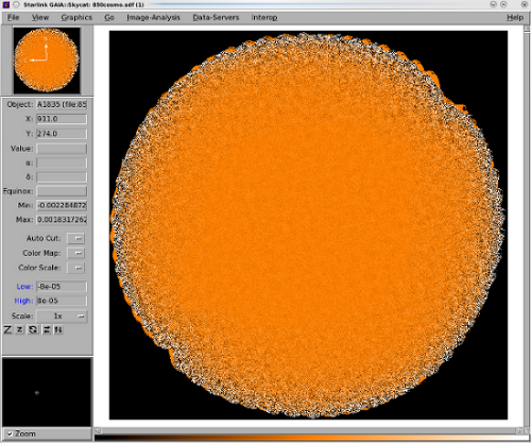
\includegraphics[width=0.48\linewidth]{sc21_850cosmo_bf}
\hspace{2mm}
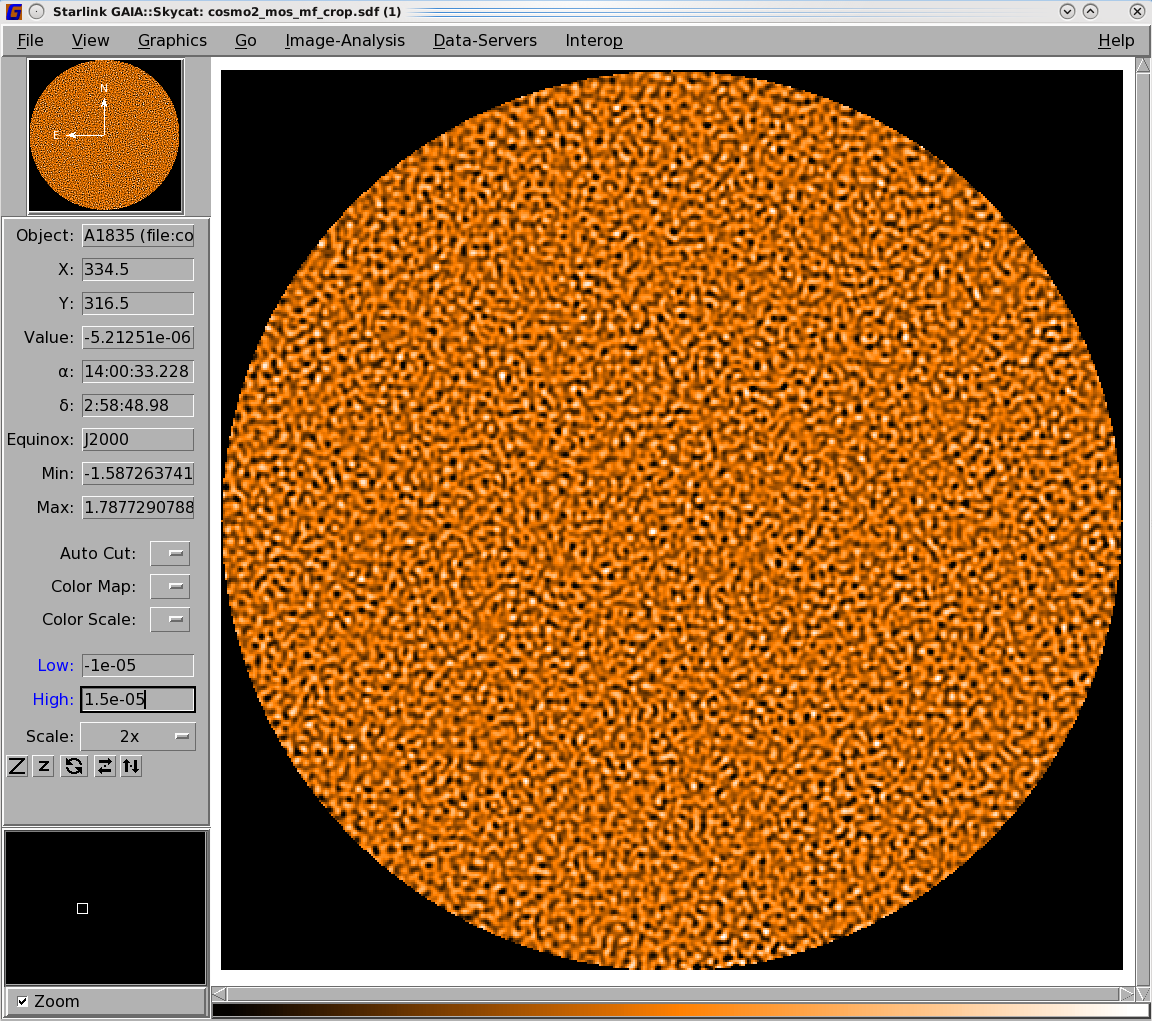
\includegraphics[width=0.48\linewidth]{sc21_850cosmo_mf_crop}
\caption[Cosmology field with the matched filter applied]{
  Reduced \textsc{pong} maps of cosmology field A1835. \textbf{Left:}
  Map reduced with \file{dimmconfig\_blank\_field.lis}.
  \textbf{Right:} Map on the left after the matched filter has been
  applied and it has been cropped.\label{fig:cosmomap}
}
\end{figure}

\textbf{Step 3: Apply the matched filter}\\
In order to optimally find sources that are the size of the telescope
beam, we apply the matched filter recipe, namely
\xref{\drrecipe{SCUBA2\_MATCHED\_FILTER}}{sun265}{SCUBA2_MATCHED_FILTER}.
We create a simple parameter file called \file{smooth.ini}:

\begin{terminalv}
[SCUBA2_MATCHED_FILTER]
SMOOTH_FWHM = 15
\end{terminalv}
where \param{SMOOTH\_FWHM~=~15} indicates that the background should be
estimated by first smoothing the map and PSF with a 15-arcsec FWHM
Gaussian. Next, the recipe is executed as follows:
%
\begin{terminalv}
% picard -recpars smooth.ini SCUBA2_MATCHED_FILTER cosmo2_mos.sdf
\end{terminalv}
%
The output of this operation is a smoothed image called
\file{cosmo3\_mos\_mf.sdf} and a cropped version is shown in the
right-hand panel of \cref{Figure}{fig:cosmomap}{figure above}. You can immediately
see the contrast to the left-hand panel which is the output from the
map-maker. A number of signal peaks now emerge as possible sources.
\\ \\
\textbf{Step 4: Crop the map}\\
Next we shall crop the map to remove the noisy edges,
in this case to a 900-arcsec radius circle. The output file will be named
\file{cosmo2\_mos\_mf\_crop.sdf}.
\begin{terminalv}
% picard CROP_JCMT_IMAGES cosmo3_mos_mf.sdf

\end{terminalv}

\starfig{sc21_850cosmo_mf_crop_snr}{}{width=0.6\linewidth}{fig:snrmask}{
  S/N map of a cosmology field}{
  Signal-to-noise map made using the \Kappa\ command \makesnr.
  The map has been scaled from 0 to $+$3.
}

\textbf{Step 5: Make an S/N map}\\
Finally, we need to find sources. The filtered map contains a
VARIANCE component, so it is easy to produce a S/N map using the
\textsc{Kappa} task \makesnr:
\begin{terminalv}
% makesnr cosmo2_mos_mf_crop cosmo2_mos_mf_crop_snr
\end{terminalv}

The resulting map, \file{cosmo2\_mos\_mf\_snr}, is shown in
\cref{Figure}{fig:snrmask}{the signal-to-noise image}. Compared with the
matched filter map the
edges no longer appear as noisy because they have been down-weighted
by the larger noise values where there were less data.
\\ \\
\textbf{Step 6: Identify sources}\\
The basic procedure for identifying sources would be to locate peaks
above some threshold S/N. The S/N image above shows peaks that are
likely to be real sources. For a start, a source appears where
expected at the 0,0 position.

But how can we check if these sources are real?
\begin{itemize}

\item One option is to split your data into mutually exclusive subsets
  and produce independent maps. Are the highest S/N peaks detected in each of
  them?
\item A second test is to compare the number of \emph{negative} peaks above
  a given S/N with the number of \emph{positive} peaks.
\end{itemize}

\subsection{Example 2 -- Advanced pipeline method}
\label{sec:jk}

Although this method is considerably simpler to execute, the products
have undergone more advanced processing than the manual method just
given. The pipeline is particularly recommended for this recipe due to
its extra analysis steps.

\textbf{Step 1: Create input file}\\
Create an file with the names of all the files you wish to process (e.g.
\file{myfiles.lis})
\\ \\
\textbf{Step 2: Run the pipeline}\\
The pipeline must first be initiated for the wavelength you are
working on. In the case below this is 850\,$\mu$m. Note that the date
does not \emph{have} to be specified when initialising the pipeline.
The pipeline is run using the
\xref{\drrecipe{REDUCE\_SCAN\_FAINT\_POINT\_SOURCES\_JACKKNIFE}}{sun264}{REDUCE_SCAN_FAINT_POINT_SOURCES_JACKKNIFE}
recipe; this uses \file{dimmconfig\_blank\_field.lis} as the
configuration file. If you wish to provide an alternative file you
will need to put the name of the new configuration file in a recipe
parameter file.  See \cref{Section}{sec:pipe}{The SCUBA-2 Pipeline}
for details.
\begin{terminalv}
% oracdr_scuba2_850 -cwd YYYYMMDD
% oracdr -loop file -files myfiles.lis -nodisplay \
-log sf FAINT_POINT_SOURCES_JACKKNIFE
\end{terminalv}

You substitute the required date for \texttt{YYYYMMDD}.
The pipeline will write out a large number of files with the following
suffices.

\begin{aligndesc}
\item[\file{sYYYYMMDD*\_fmos}]
The map for each observation

\item[\file{sYYYYMMDD*\_mappsf}] The map for each observation with an
  artificial point source added at the map centre

\item[\file{gsYYYYMMD*\_wmos}] The co-add of all the \file{\_fmos}
  files

\item[\file{gsYYYYMMD*\_whiten}] The whitened version of \file{\_wmos}

\item[\file{gsYYYYMMD*\_cal}] The calibrated version of
  \file{\_whiten}

\item[\file{gsYYYYMMD*\_mf}] The matched-filtered version of
  \file{\_cal}
\end{aligndesc}

\drrecipe{FAINT\_POINT\_SOURCES\_JACKKNIFE} is a recipe designed to
process blank field/extra-galactic data. The recipe uses a
\htmladdnormallink{jack-knife}{http://en.wikipedia.org/wiki/Jackknife_resampling}
method to remove low-spatial frequency noise and generate a matched
filter output map.

The recipe processes each observation twice, a standard reduction
first, then a re-run with a fake point source added to the time
series. This produces a co-added signal map (\file{\_wmos}) and a
coadded PSF map (\file{\_mappsf}).

\begin{tip}
The recipe name \drrecipe{FAINT\_POINT\_SOURCES\_JACKKNIFE} can be used
interchangably with  \drrecipe{REDUCE\_SCAN\_FAINT\_POINT\_SOURCES\_JACKKNIFE}.
\end{tip}


After the map-maker has completed, the recipe will call
\xref{\drrecipe{SCUBA2\_JACKKNIFE}}{sun265}{SCUBA2_JACKKNIFE}. This
routine divides the observations into two groups (odd and even) which
are co-added and then subtracted to create a jack-knife map. This map
contains only noise with no contribution from astronomical signal. The
angular power spectrum of this map is then used to estimate and remove
the residual 1/\emph{f} noise from the signal map and the PSF map;
this is the whitening step. The whitened jack-knife map is run through
\xref{\drrecipe{SCUBA2\_MATCHED\_FILTER}}{sun265}{SCUBA2_MATCHED_FILTER}
using the whitened PSF map as the PSF input. It is this matched filter
map which will be of most interest to users.

See \pipelinesun\ for more information on
\drrecipe{REDUCE\_SCAN\_FAINT\_POINT\_SOURCES\_JACKKNIFE} and all other pipeline
recipes.
\\ \\
\textbf{Step 3: (Optional) Re-run \drrecipe{SCUBA2\_JACKKNIFE}}\\
You may wish to run the \drrecipe{SCUBA2\_JACKKNIFE} step again
independently from the pipeline. If your final map does not look as
expected you might first examine the individual mosaics from the
pipeline (\file{\_fmos}), one of these observations might show visible
artefacts that you wish to exclude from the co-add. The size of the
region in the jack-knife image which is used to do the whitening step
is determined automatically, but the method may fail if the box is too
small.

If you decide to re-run this step you first co-add all the
\file{\_mappsf} files to create a coadded PSF using the \picard\ recipe
\xref{\drrecipe{MOSAIC\_JCMT\_IMAGES}}{sun265}{MOSAIC_JCMT_IMAGES}.
\begin{terminalv}
% picard MOSAIC_JCMT_IMAGES *_mappsf
\end{terminalv}
Next create a parameter file (\file{recpars.lis}) for the jack-knife
recipe (\drrecipe{SCUBA2\_JACKKNIFE}) containing the following lines.
\begin{terminalv}
[SCUBA2_JACKKNIFE]
PSF_MATCHFILTER = <name_of_above_coadded_PSF>.sdf
\end{terminalv}
Another option for this parameter file is \param{WHITEN\_BOX} to set the
size of the region used to calculate the angular power spectrum.
Finally run \drrecipe{SCUBA2\_JACKKNIFE}.
\begin{terminalv}
% picard -log sf -nodisplay -recpars recpars.lis SCUBA2_JACKKNIFE *fmos.sdf
\end{terminalv}
This will create files beginning with \file{pgYYYMMDD}$\ldots$ that
should have the same suffices as above: \file{\_wmos},
\file{\_whiten}, \file{\_cal}, and \file{\_mf}.



\section{\xlabel{Galactic}Extended galactic sources}
\label{sec:bright_ex}

This example is concerned with recovering bright extended emission.
The signal from extended emission varies slowly as seen by the array
passing over it. It thus appears at lower frequencies in the power
spectrum and complicates the high-pass filter selection. Too harsh a
filter will make flat maps but any extended emission will have been
removed in doing so.
\\ \\
\textbf{Step 1: Running the map-maker}
\vspace{0.2cm}\\
We run the map-maker using \file{dimmconfig\_bright\_extended.lis};
we have also specified a couple of overrides on the command
line---\xparam{MAPTOL}{maptol}~=~0.04 is slightly more stringent than default and
\xparam{AST.ZERO_SNR}{ast.zero\_snr}~=~3.5 constrains everything below
3.5\,$\sigma$ to zero.

In this example we give the map-maker a file containing a list of the
input files (\file{filelist.txt}) and
\file{dimmconfig\_bright\_extended.lis} is in the local directory.

\begin{terminalv}
% makemap in=^filelist.txt 850galactic \
          config='"^dimmconfig_bright_extended.lis,maptol=0.04,ast.zero_snr=3.5"'
\end{terminalv}
The resulting map is shown in \cref{Figure}{fig:galmakemap}{the figure below}.

\starfig{sc21_gal_11}{[t!]}{width=0.6\linewidth}{fig:galmakemap}{
  Galactic example: initial reduction using \file{dimmconfig\_bright\_extended.lis}}{
  The output from the map-maker using \file{dimmconfig\_bright\_extended.lis}.
}

\textbf{Step 2: Generating an external mask}
\vspace{0.2cm}\\
Next we create an external mask from the output of \makemap. Here we
follow the steps outlined in \cref{Section}{sec:maskbe}{Using external
masks}.

\begin{terminalv}
% makesnr 850map 850map_snr
\end{terminalv}

This S/N map is thresholded to set everything below 3\,$\sigma$ to 0 and
everything above to 1.

\begin{terminalv}
% thresh 850map_snr 850map_mask thrlo=3 newlo=0 thrhi=3 newhi=1
\end{terminalv}
The thresholded map is shown in the left-hand panel of
\cref{Figure}{fig:mask}{this figure}. The next step is to smooth this map
by convolving it with a Gaussian of 16\,arcsec. For this we use a factor
of 4 for the FWHM parameter.

\begin{terminalv}
% gausmooth 850map_mask 850map_mask_sm fwhm=4
\end{terminalv}

We threshold the map again to produce our mask. In this case all
values below our threshold are set to `bad'. The smoothed map now
has values scaled between 0 and 1, we set our threshold at 0.02 to
include more of the emission beyond the 3\,$\sigma$ edge.
\begin{terminalv}
% thresh 850map_mask_sm 850map_mask_zm thrlo=0.02 newlo=bad thrhi=0.02 newhi=1
\end{terminalv}
The final mask is shown in the right-panel of \cref{Figure}{fig:mask}{the figure below}.
Note how it encompasses more emission and has softer edges than the
first threshold map. \\

\begin{figure}[t]
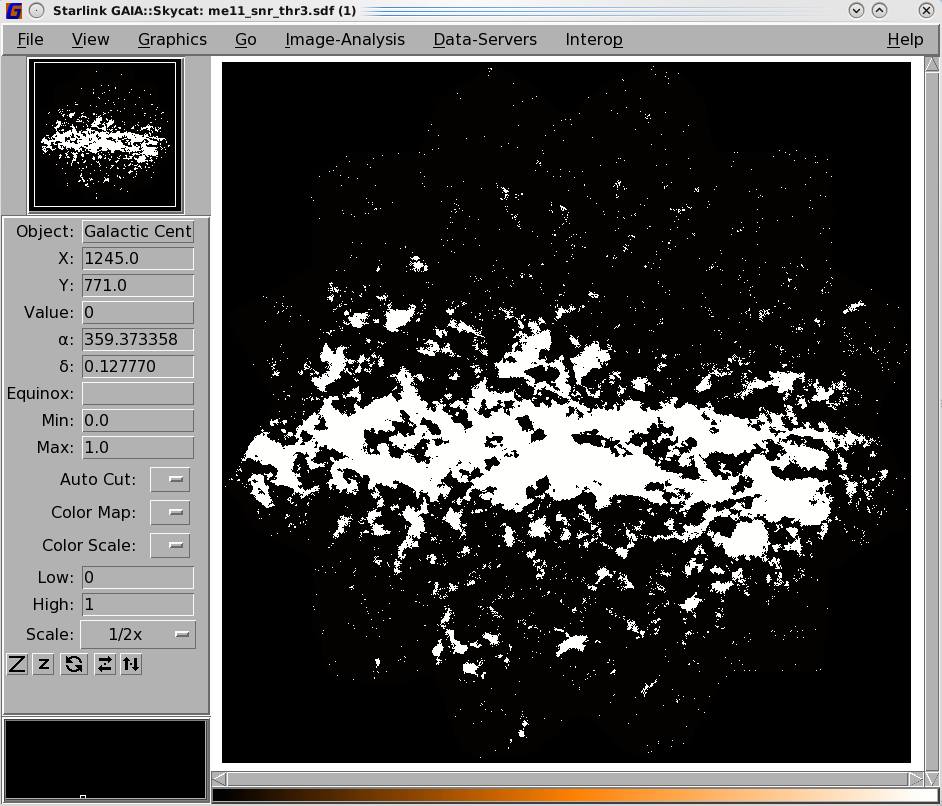
\includegraphics[width=0.475\linewidth]{sc21_gal_mask1}
\hspace{2mm}
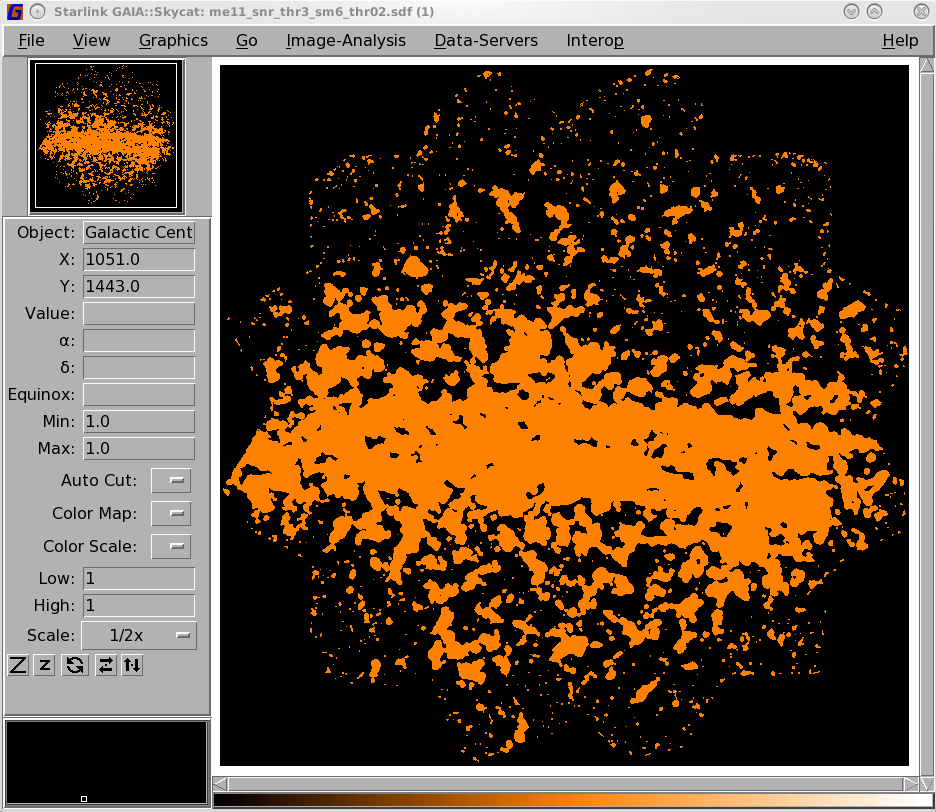
\includegraphics[width=0.475\linewidth]{sc21_gal_mask2}
\caption[Galactic example: thresholded SNR map and smoothed map]{
  \textbf{(Left)} The initial mask created by thresholding 850map\_snr
  to 3$\sigma$. \textbf{(Right)} Second mask made by thresholding the
  smoothed map to 0.02.\label{fig:mask}
}
\end{figure}


\textbf{Step 3: Re-running the map-maker with an external mask supplied}
\vspace{0.2cm}\\
As a last step the map is re-made with this mask supplied as an external
file. For this run we apply the additional parameters in a
personalised configuration file, \file{mydimmconfig.lis}.
\begin{terminalv}
% makemap in=^filelist.txt 850galactic \
          config=^mydimmconfig.lis ref=850map_mask_zm
\end{terminalv}

The configuration file, \file{mydimmconfig.lis}, has the following
format---note how it is based on
\file{dimmconfig\_bright\_extended.lis}. It has decreased the
convergence parameter to \xparam{MAPTOL}{maptol}~=~0.03 but increased the number
of iterations to compensate as 40 is unlikely to be sufficient.
\begin{terminalv}
^$STARLINK_DIR/share/smurf/dimmconfig_bright_extended.lis
numiter = -100
noisecliphigh = 10.0
maptol = 0.03
ast.zero_mask=1
ast.zero_snr = 0
\end{terminalv}

\textbf{Step 4: Cropping the map}
\vspace{0.2cm}\\
We now crop the map to remove the noisy edges using the \picard\ recipe
\drrecipe{CROP\_JCMT\_IMAGES}. To determine what to trim we can look
at the exposure-time image with \gaia.  See
\cref{Figure}{fig:exptime}{the exposure time image}.

\starfig{sc21_gal_exptime}{[h!]}{width=0.7\linewidth}{fig:exptime}{
  Galactic example: exposure time map}{
  The exposure-time image of the science map from \cref{Figure}{fig:galmakemap}{
  our example map}. You can right-click and drag the mouse
  between two points to measure the distance. Here we see the exposure
  time dropping off sharply at a radius of 30\,arcmin. A non-default
  colour scale has been chosen to illustrate the morphology.
}

The exposure-time map shows a sharp drop off at a radius of 30\,arcmin.
We can thus specify a parameter file like below.
\begin{center}
\begin{terminalv}
[CROP_JCMT_IMAGES]
MAP_RADIUS = 1800
\end{terminalv}
\end{center}

\begin{terminalv}
% picard CROP_JCMT_IMAGES 850galactic.sdf
\end{terminalv}
The final cropped map is shown in \cref{Figure}{fig:crop_map}{this plot}.
Compared with the first map out of the map-maker
(\cref{Figure}{fig:galmakemap}{first map}),
slightly more of the faint extended emission is apparent.

One of the challenges facing this type of reduction is the need to
account for both faint extended structure and very bright sources in
the same map. You may find some degree of bowling remains around the
brightest sources.

There are areas you may wish to experiment with. One is to adjust the
filtering. Another option is to supply an external mask from
a different dataset, e.g. a
\htmladdnormallink{Herschel}{http://herschel.esac.esa.int/} map.
See \cref{Chapter}{sec:tweak}{Tailoring Your Reduction} for further
discussion.

\starfig{sc21_gal12_crop}{[b!]}{width=0.65\hsize}{fig:crop_map}{
  Galactic example: cropped final map}{
  The final cropped, reduced map from the map-maker run with
  an external mask supplied.
}


\clearpage
